\documentclass[a4paper,10pt]{ica2013_2}
\usepackage[utf8x]{inputenc}
\usepackage{xcolor}
\usepackage{titlesec}
\usepackage{natbib}




\begin{document}
\section{First level heading (heading 1)}
This is the standard font and layout for the individual paragraphs.  The style is called "Paragraph."  Replace this text with your text.
\subsection{Second Level Heading (Heading 2) with Each Initial Letter Capitalized (Note: 
prepositions and articles should be lowercase)}
This is the standard font and layout for the individual paragraphs.  The style is called "Paragraph."  Replace this text with your text.
\subsubsection{Third Level Heading (Heading 3) with Each Initial Letter Capitalized (Note: prepositions and articles should be lowercase)}
Below is an example to place a new equation.
\begin{equation}
 \frac{d F_1}{d\omega}=SAm_2\,\cos \omega
\end{equation}
Some references \citep{bacon2000hot,hamilton1837third, kulvait2012nonlinear} are cited here as sample refernces. These references are included in the sample bibtex file attached with this file.

Sample table below
\begin{table}[!h]
\centering
\caption{Center the caption above the Table.  Tables should have top and bottom 
rules, and a rule separating the column heads from the rest of the table only.  Do not display all grid lines}\label{table:aerodynamic_results}
 \begin{tabular}{ccc}
\hline
\textbf{Column Header Goes Here} & \textbf{Column Header Goes Here}  & \textbf{Column Header Goes Here}\\
\hline
Numerical  & 0.751  & 0.08\\
Experimental & 0.750 & 0.071\\
\hline
 \end{tabular}
\end{table}

You can also add figures in EPS (using latex) or PDF format (using pdflatex). Pictures can also be imported as PNG files if you use pdflatex. See for example Fig.~
\begin{figure}[!h]
\centering
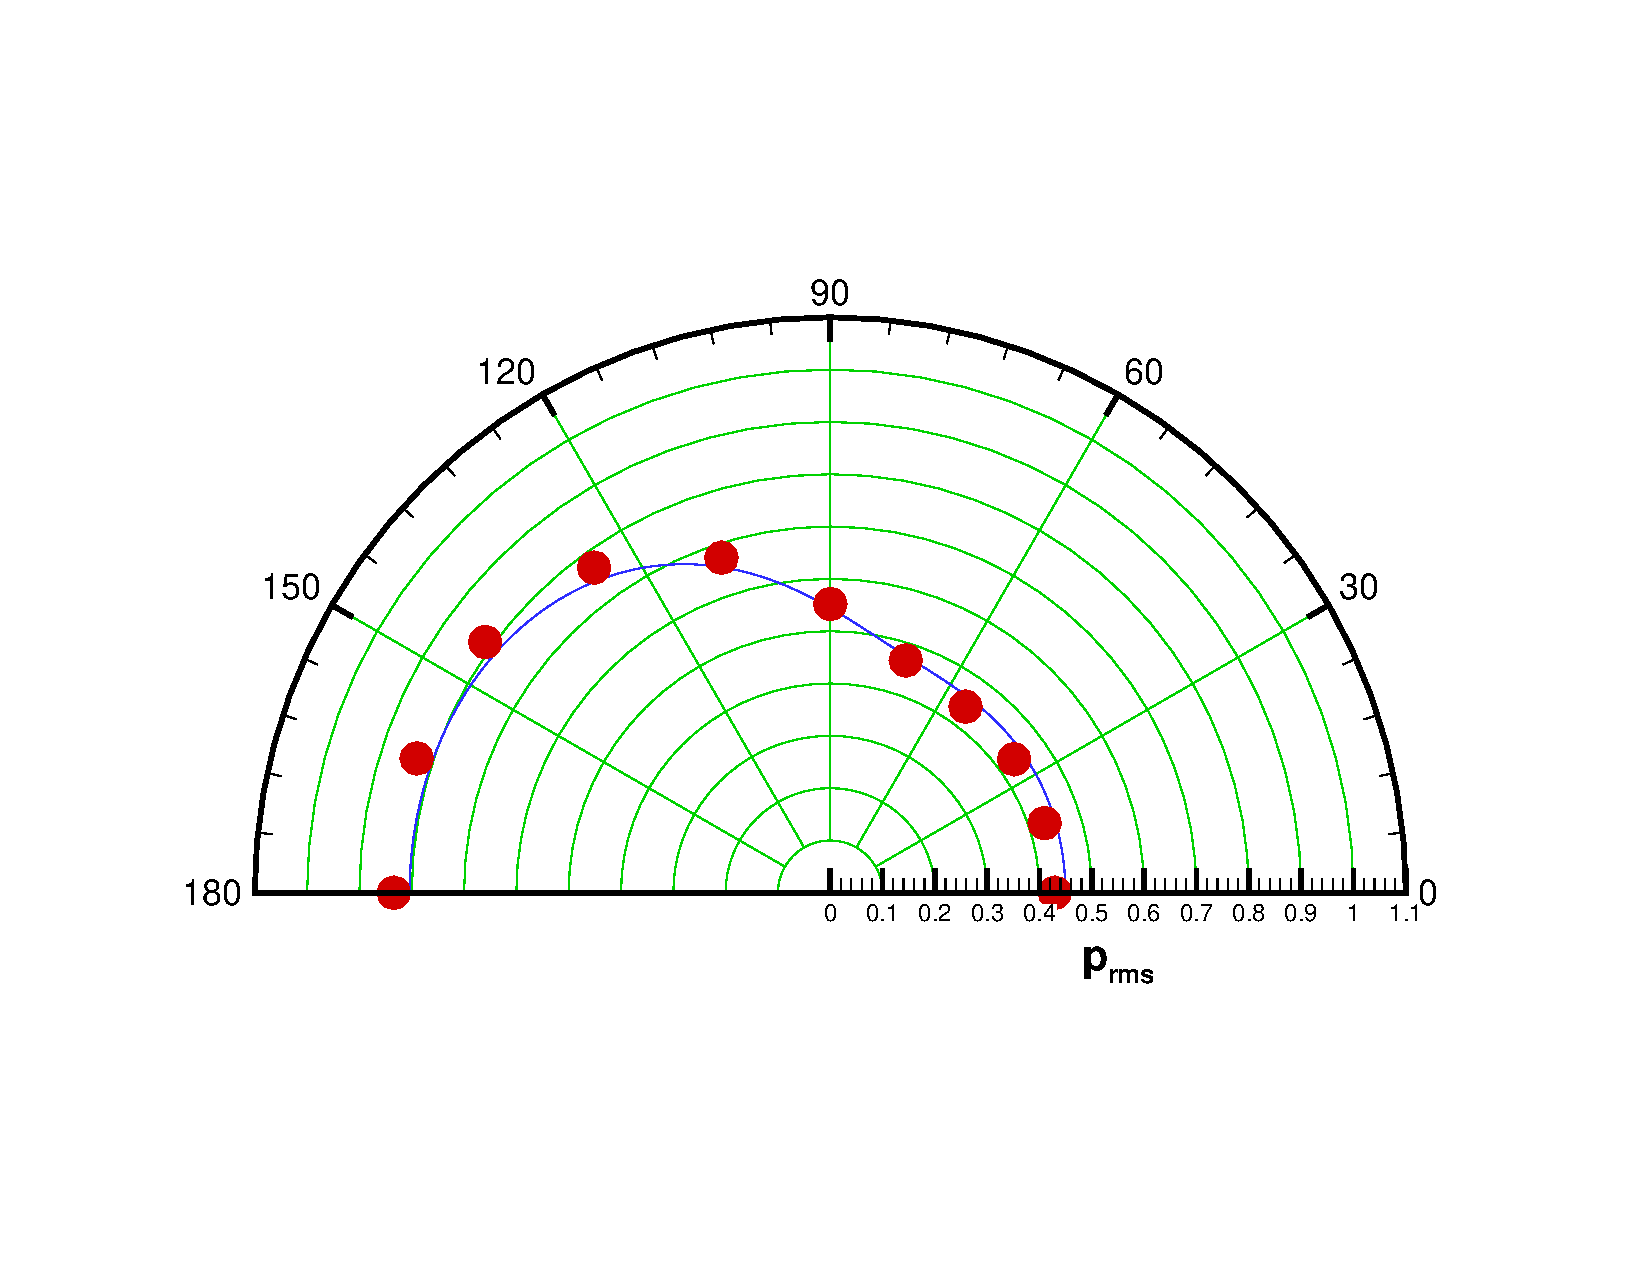
\includegraphics[width=0.45\textwidth]{sample_fig.pdf}
\caption{This is a sample figure. You can put the caption here.}\label{fig:sample_fig}
\end{figure}

\section*{ACKNOWLEDGMENTS}
Acknowledgments go here. Note that you must use \begin{verbatim}\section*\end{verbatim} command to remove the section numbering.

The references in the next section should follow either \textit{JASAnum} or \textit{JASAAuthyear} bibtex style. If using \textit{JASAAuthyear}, use the \textit{natbib} package by uncommenting the respective command in the header of the  latex file.
%\bibliographystyle{jasanum}
\bibliographystyle{jasaauthyear}

\bibliography{template}
\end{document}
